\chapter{Implementacija i korisničko sučelje}
		
		
		\section{Korištene tehnologije i alati}
		\bigskip
			
		\textbf{\textit{izrada aplikacije}}
		\bigskip
		\bigskip
		
			 \textit{ Po modelu klijent - poslužitelj, "klijentska strana aplikacije" (front-end) realizirana je pomoću Reacta\footnote{\url{https://reactjs.org}} u razvojnom okruženju Visual Studio Code\footnote{\url{https://code.visualstudio.com}} uz korištenje jezika Javascript\footnote{\url{https://www.javascript.com}} .  React je Javascript biblioteka otvorenog koda za izgradnju korisničkih sučelja temeljenih na komponentama korisničkog sučelja. Za implementaciju "poslužiteljske strane" (back-enda) korišten je Spring Boot\footnote{\url{https://spring.io/projects/spring-boot}} zasnovan na razvojnom okviru Spring\footnote{\url{https://spring.io}} u razvojnom okruženju Eclipse\footnote{\url{https://www.eclipse.org}} uz korištenje jezika Java\footnote{\url{https://www.java.com/en/}} . Arhitektura sustava je oblikovana objektno usmjereno pa iz tog razloga koristimo Javu kao objektno orijentirani programski jezik. Spring Boot je radni okvir temeljen na Javi. Za prikladno strukturiranje i spremanje podatka korištena je relacijska baza podataka, implementirana pomoću PostgreSQL-a\footnote{\url{https://commandprompt.com/education/how-to-download-and-install-postgresql/}} . Relacijska baza podataka nam osigurava laku manipulaciju podacima te određenu razinu sigurnosti.}
			 
		\bigskip
			\bigskip
			 
			 \textbf{\textit{izrada dokumentacije}}
			 \bigskip
			 

    				 \textit{Za izradu dokumentacije korišten je markup jezik LaTeX\footnote{\url{https://www.latex-project.org}} (slično kao HTML). LaTeX datoteka je tip tekstualne datoteke koja nam olakšava rad sa sustavom za verzioniranje. Korišten je TeXstudio\footnote{\url{https://www.texstudio.org/}}, uređivač teksta koji je prilagođen LaTeXu. Za kreiranje pdf dokumenta iz LaTeX dokumenta korišten je TeXLive\footnote{\url{https://www.tug.org/texlive/}} . Za izradu UML dijagrama korišten je online alat VisualParadigm\footnote{\url{https://online.visual-paradigm.com/drive/\#diagramlist:proj=0&dashboard}}. }
				 \bigskip
			 
			 \textbf{\textit{ostalo}}
			 \bigskip
			 
				 \textit{	Komunikacija u timu realizirana je korištenjem aplikacije WhatsApp\footnote{\url{https://www.whatsapp.com}} i Discord\footnote{\url{https://discord.com}}. Kao sustav za upravljanje izvornim kodom korišten je Git\footnote{\url{https://git-scm.com/}} . Udaljeni repozitorij projekta dostupan je na web platformi GitLab \footnote{\url{https://gitlab.com/}} .}
			 	
		\newpage
		\section{Ispitivanje programskog rješenja}

			
			 \textit{Za testiranje funkcionalnosti komponenti i sustava korišteni su Selenium WebDriver i Selenium IDE ekstenzija za Chrome preglednik. }
	
			
			\subsection{Ispitivanje komponenti}
			\textit{Na slikama 5.1,5.2 i 5.3 prikazani su unit testovi uz korištenje Selenium WebDriver podrške.  Slika 5.4 omogućava uvid u uspješnost izvršavanja testova.}
		\newline
		\newline
			\textit{Na slici 5.1 možemo vidjeti testiranje metode dohvatiKlijenta iz implementacije klijent servisa i uspješno dohvaćanje korisnika. }
			\begin{figure}[H]
				\centering
				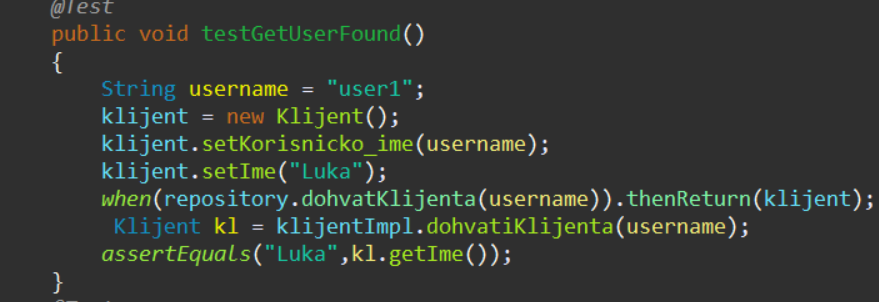
\includegraphics[width=\textwidth,height=8cm]{slike/slike_testova/JUNIT/test1.PNG}
				\caption{Dohvaćanje postojećeg korisnika}
				\label{fig:my_label}
			\end{figure}
		
		
		\newpage
		
		\textit{
			Slika 5.2 prikazuje pokušaj dohvaćanja klijenta koji nije u repozitoriju što vraća null vrijednost. }
		\begin{figure}[H]
			\centering
			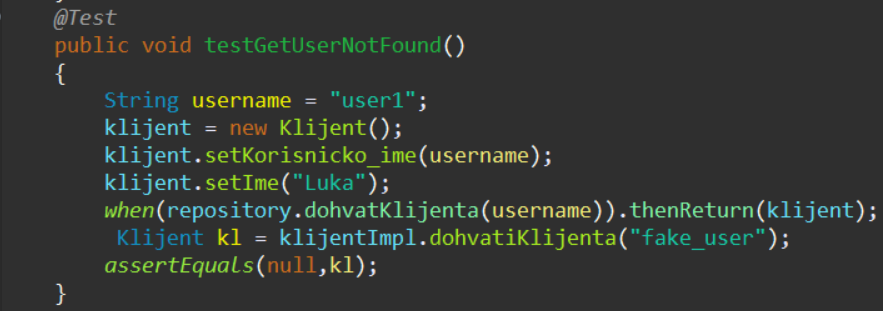
\includegraphics[width=\textwidth,height=8cm]{slike/slike_testova/JUNIT/test2.PNG}
			\caption{Dohvaćanje nepostojećeg korisnika}
			\label{fig:my_label}
		\end{figure}
	
	\textit{
		Slika 5.3 prikazuje slučaj brisanja korisnika koji nije prethodno dodan u repozitorij i stoga brisanje nije moguće. Povratna vrijednost metode je null. }
	\begin{figure}[H]
		\centering
		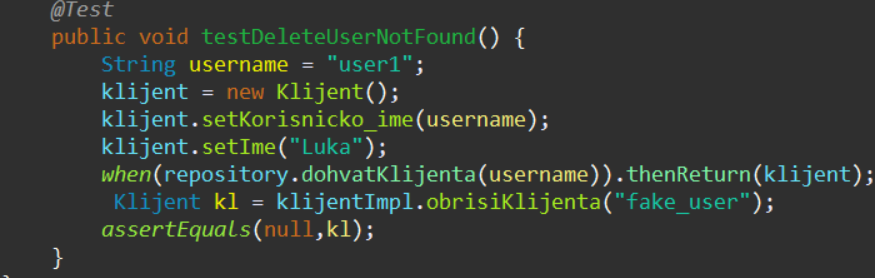
\includegraphics[width=\textwidth,height=8cm]{slike/slike_testova/JUNIT/test3.PNG}
		\caption{Brisanje nepostojećeg korisnika}
		\label{fig:my_label}
	\end{figure}
			
			\newpage
			\begin{figure}[H]
				\centering
				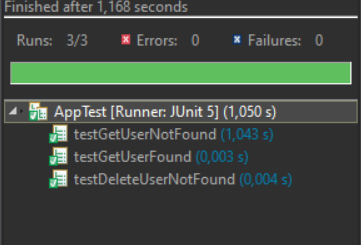
\includegraphics[width=\textwidth,height=8cm]{slike/slike_testova/JUNIT/results.PNG}
				\caption{Rezultati JUNIT testova}
				\label{fig:my_label}
			\end{figure}
			
			\subsection{Ispitivanje sustava}
			
			 \textit{Na slikama 5.5 do 5.11 prikazano je testiranje sustava i rezultati dobiveni korištenjem Selenium IDE. }
			 
			\newline
			\textit{
				Slika 5.5 prikazuje pokušaj izrade kluba koji već postoji. }
			\begin{figure}[H]
				\centering
				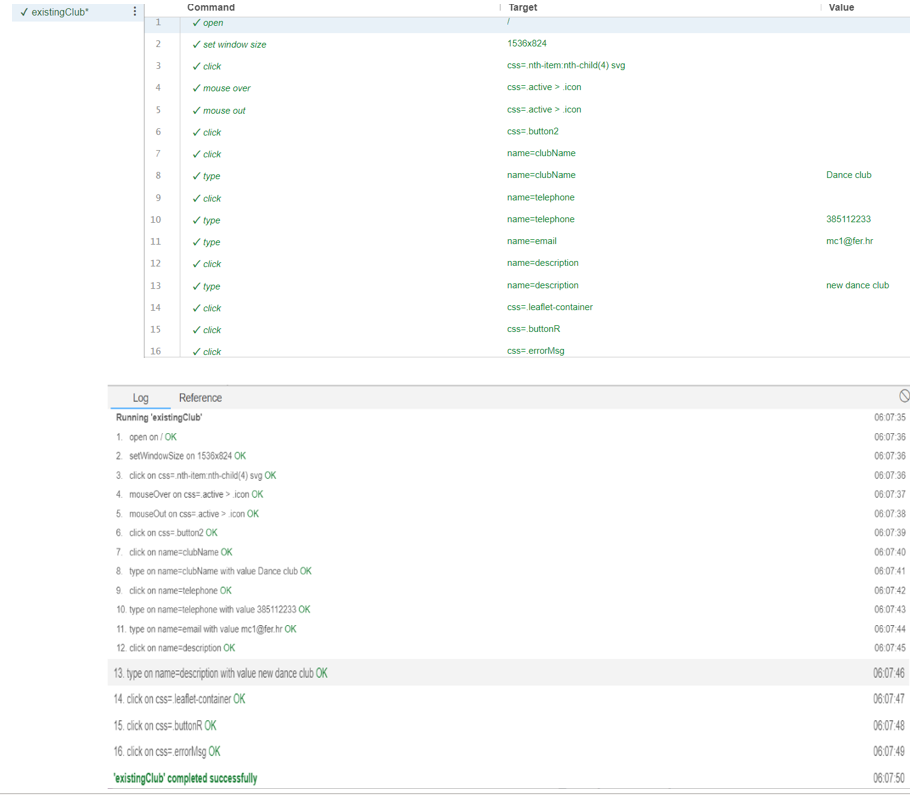
\includegraphics[width=\textwidth,height=8.5cm]{slike/slike_testova/SELENIUM_IDE/1.PNG}
				\caption{Kreiranje postojećeg kluba}
				\label{fig:my_label}
			\end{figure}
		\newpage
		\textit{
			Slika 5.6 prikazuje pokušaj prijave korisnika za instruktora plesa bez priloženih trenerskih akreditiva. }
		\begin{figure}[H]
			\centering
			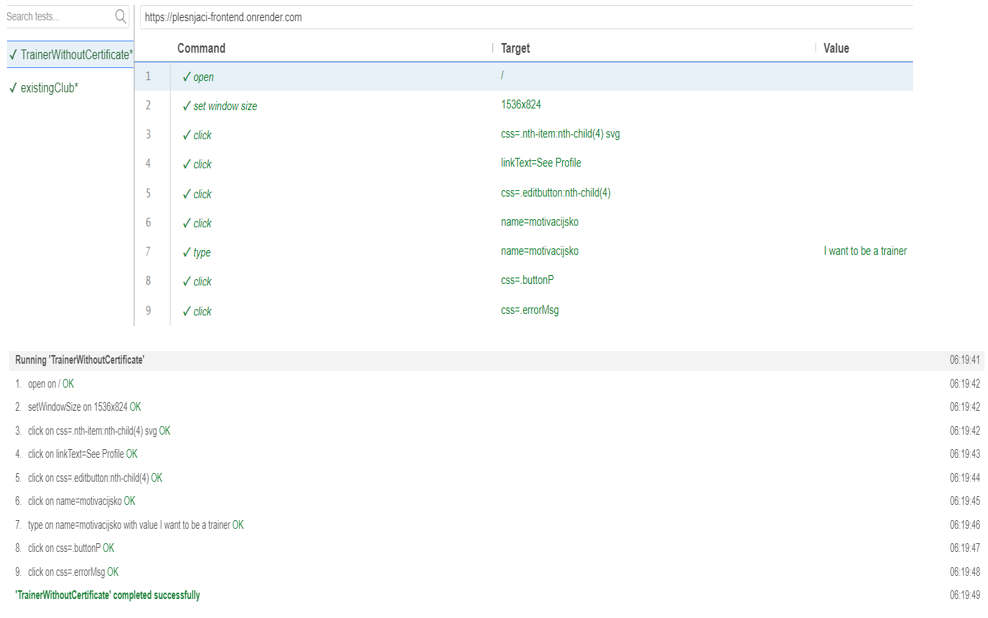
\includegraphics[width=\textwidth,height=8.5cm]{slike/slike_testova/SELENIUM_IDE/2.PNG}
			\caption{Pokušaj prijave za instruktora}
			\label{fig:my_label}
		\end{figure}
	\textit{
		Na slici 5.7 vidimo pokušaj registracije korisnika koji već postoji u sustavu i stoga nije moguć. }
	\begin{figure}[H]
		\centering
		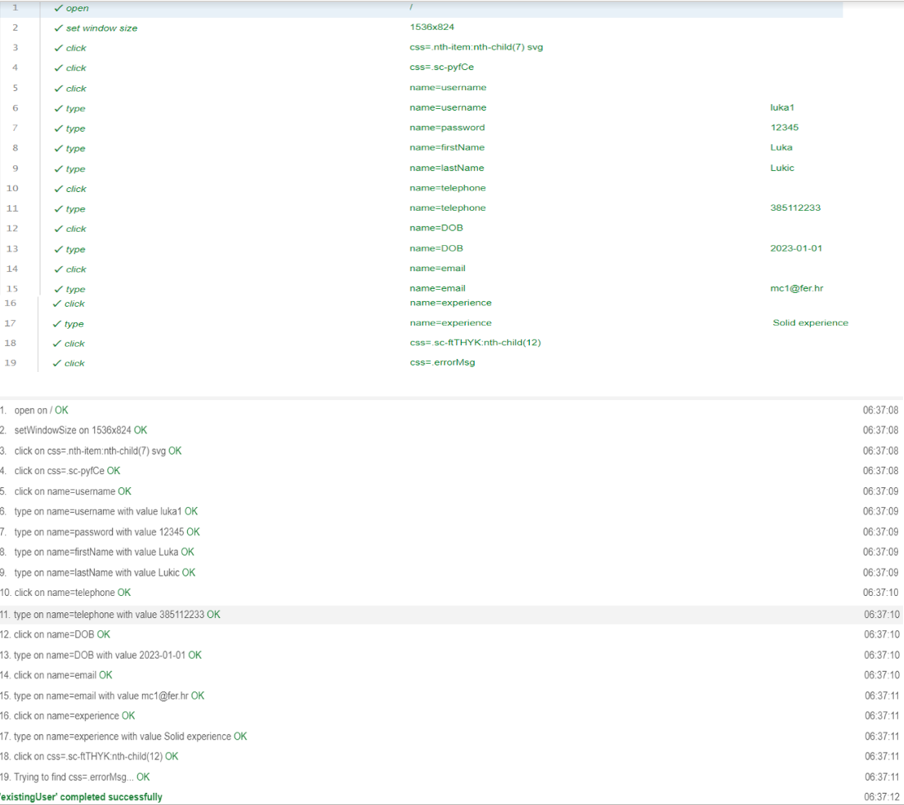
\includegraphics[width=\textwidth,height=8cm]{slike/slike_testova/SELENIUM_IDE/3.PNG}
		\caption{Nedozvoljeni pokušaj registracije}
		\label{fig:my_label}
	\end{figure}
	\newpage
	\textit{
		Slika 5.8 pokazuje pokušaj izrade tečaja bez specificiranja o kojoj vrsti plesa se radi što nije dozvoljeno. }
	\begin{figure}[H]
		\centering
		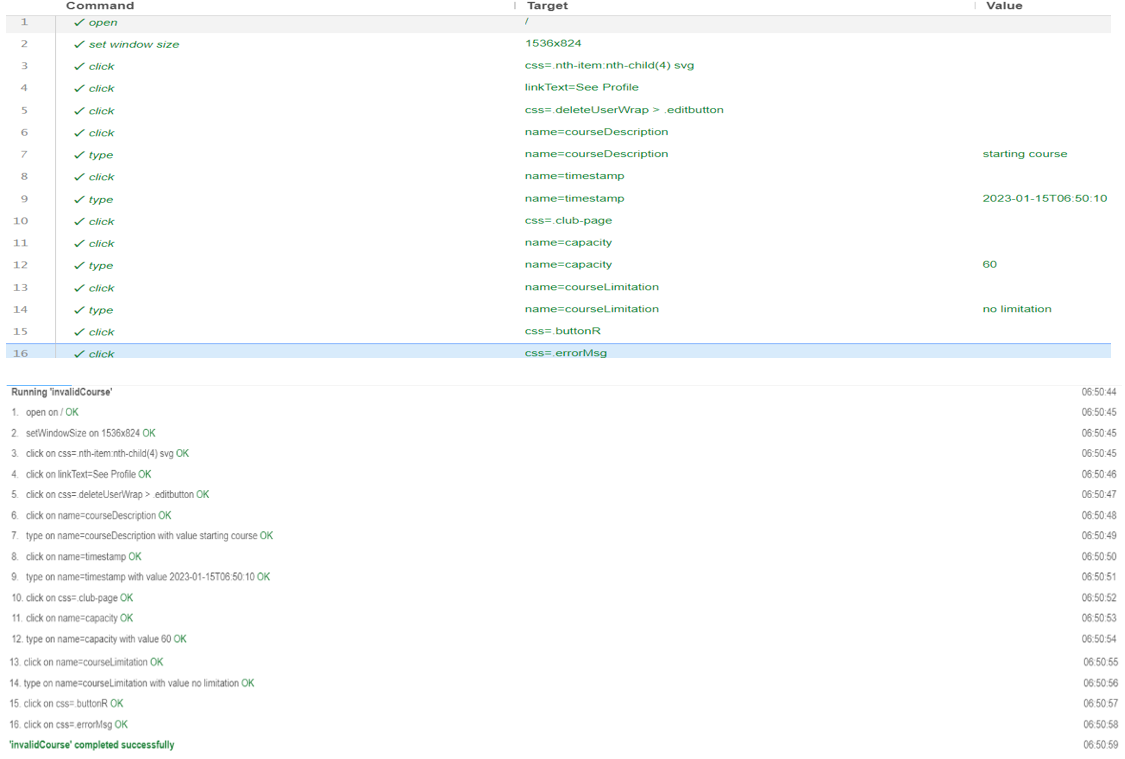
\includegraphics[width=\textwidth,height=8cm]{slike/slike_testova/SELENIUM_IDE/4.PNG}
		\caption{Nedozvoljeno kreiranje tečaja}
		\label{fig:my_label}
	\end{figure}
\textit{
	Slika 5.9 prikazuje pokušaj izmjene događaja uz navođenje neispravnog formata datuma što uzrokuje grešku. }
\begin{figure}[H]
	\centering
	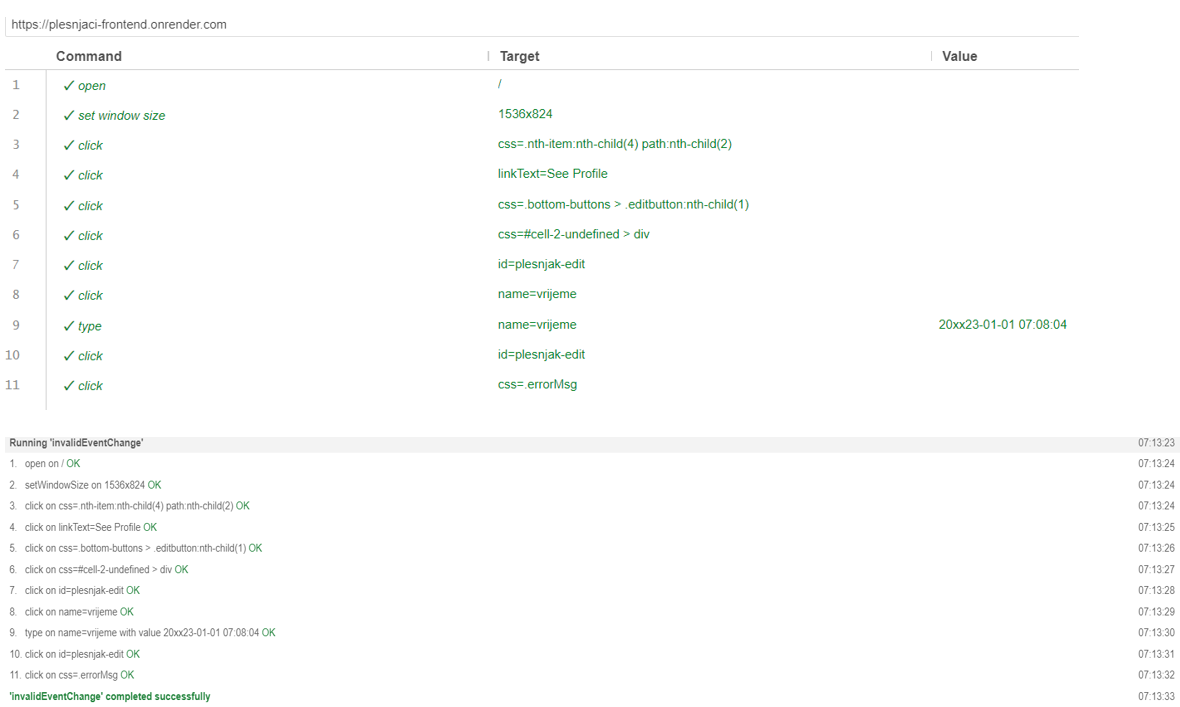
\includegraphics[width=\textwidth,height=8cm]{slike/slike_testova/SELENIUM_IDE/5.PNG}
	\caption{Nepravilna izmjena datuma}
	\label{fig:my_label}
\end{figure}
\newpage
	\textit{
		Na slici 5.10 prikazano je ispravno brisanje korisnika uz potvrdu. }
	\begin{figure}[H]
		\centering
		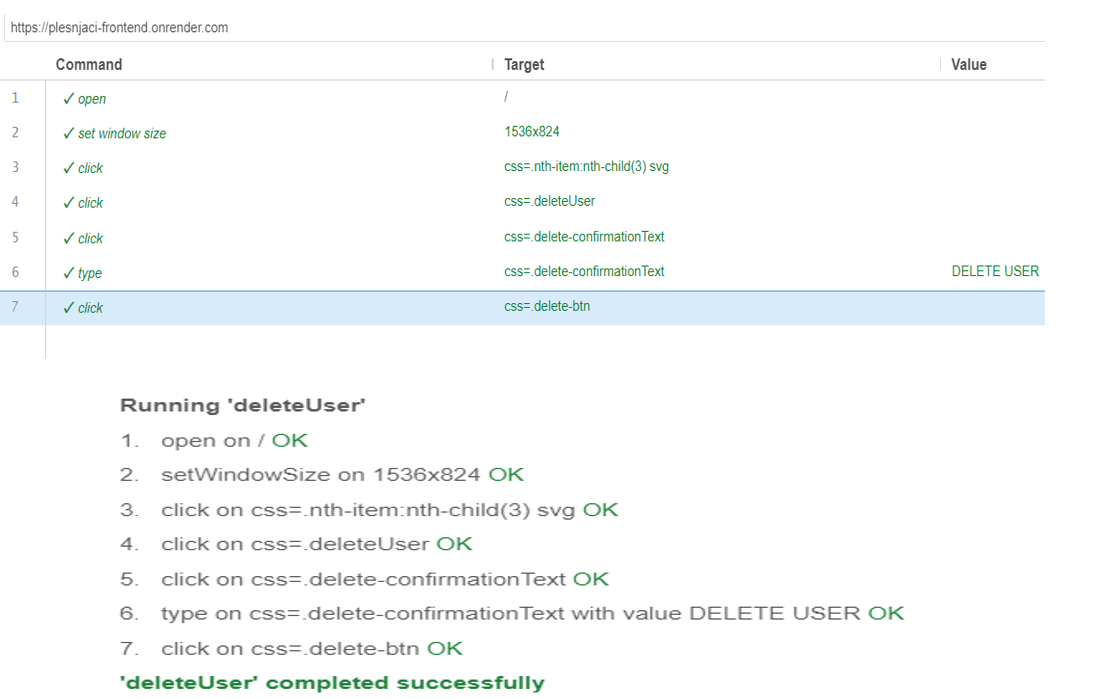
\includegraphics[width=\textwidth,height=8cm]{slike/slike_testova/SELENIUM_IDE/6.PNG}
		\caption{Ispravno brisanje korisnika}
		\label{fig:my_label}
	\end{figure}
\textit{
	Slika 5.11 sadržava pokušaj registracije korisnika uz unošenje nedozvoljenog tipa informacija. }
\begin{figure}[H]
	\centering
	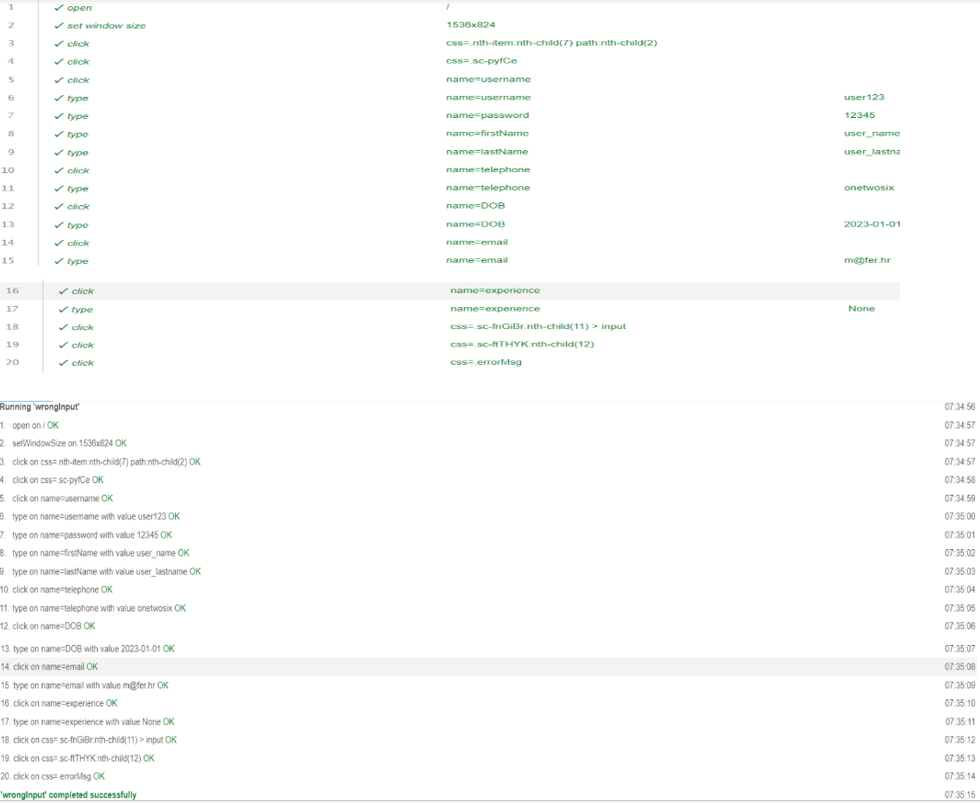
\includegraphics[width=\textwidth,height=9.5cm]{slike/slike_testova/SELENIUM_IDE/7.PNG}
	\caption{Nedozvoljen tip podataka}
	\label{fig:my_label}
\end{figure}
			\eject 
		
		
		\section{Dijagram razmještaja}
		\bigskip
		\bigskip
		
			\textit{Dijagram razmještaja opisuje topologiju sustava, odnos sklopovskih i programskih dijelova. Slika 5.1 prikazuje specifikacijski dijagram razmještaja. Na poslužiteljskom računalu nalazi se web aplikacija i baza podataka. Klijenti koriste web preglednik kako bi pristupili aplikaciji. Sustav funkcionira po modelu "klijent - poslužitelj". Klijent zahtjeva uslugu od strane poslužitelja, šalje mu HTTP zahtjev i očekuje odgovor. Poslužitelj obrađuje zahtjeve te šalje odgovor klijentu. Poslužitelj je također zadužen za komunikaciju s bazom podataka. }

			\bigskip
			\bigskip
			
			\begin{figure}[H]
				\centering
				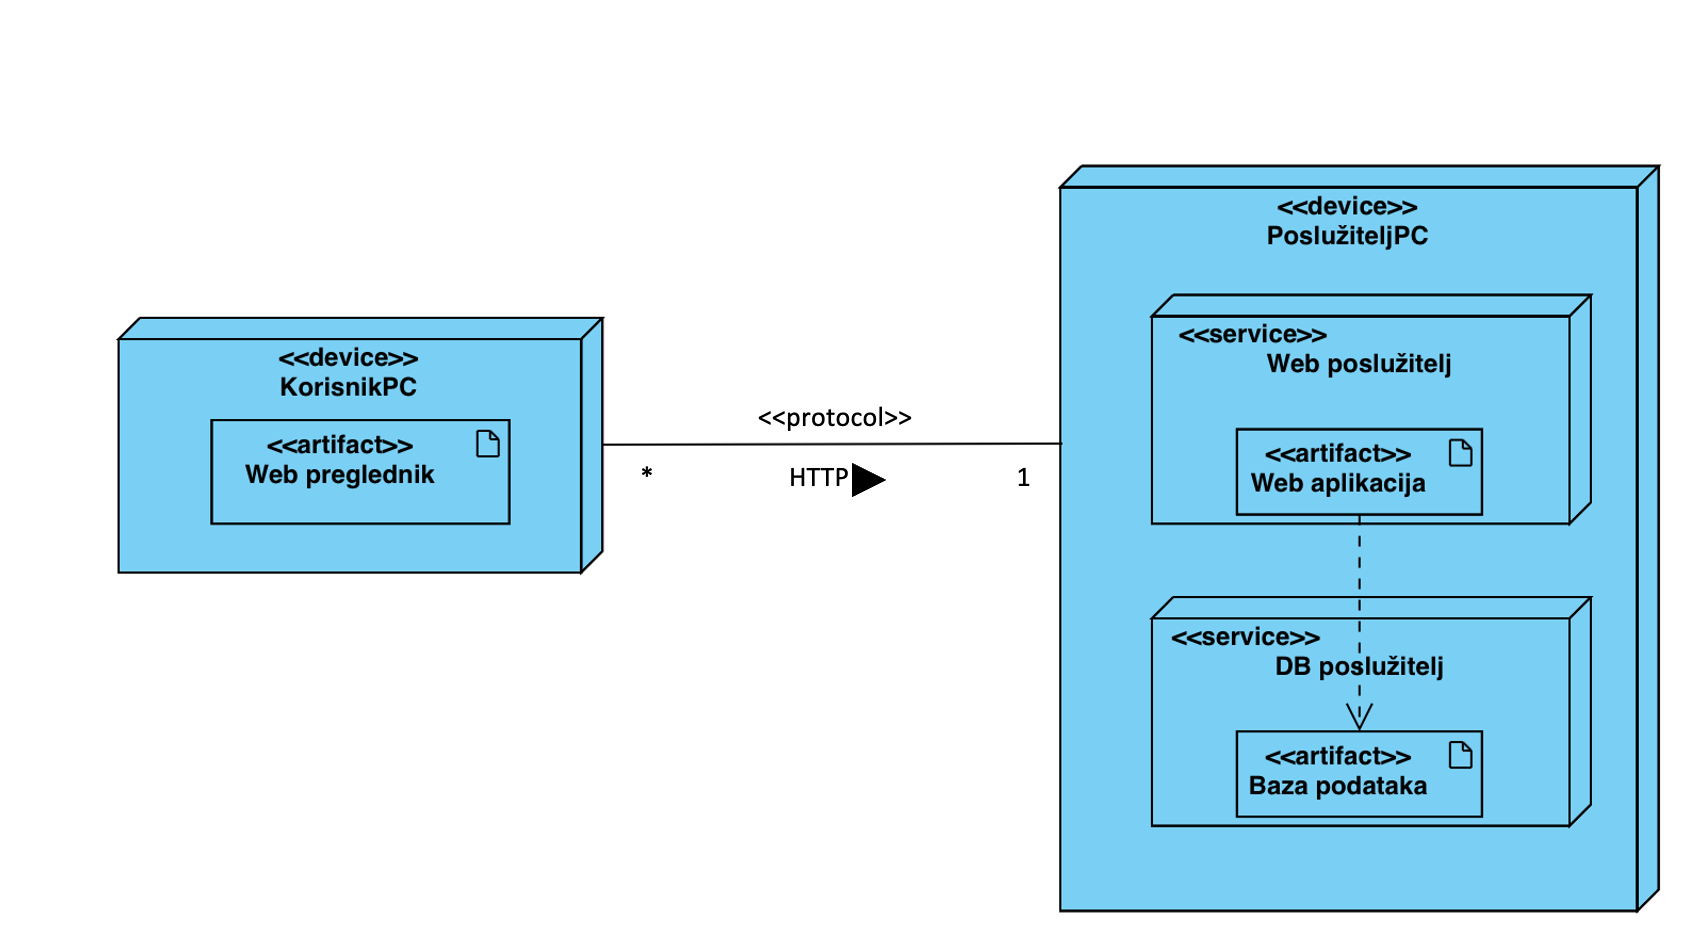
\includegraphics[width=\textwidth]{slike/dijagram_razmjestaja.png}
				\caption{Specifikacijski dijagram razmještaja}
				\label{fig:my_label}
			\end{figure}
		
		
		\newpage
		
		
		\section{Upute za puštanje u pogon}
		
		\textbf{\textit{Općenito}}\\
			\textit{Za puštanje aplikacije u pogon koristili smo Render cloud servis za hostanje baze podatka te backend i frontend aplikacija. Odabrali smo Render zato što pruža mogućnost automatske izgradnje aplikacije svaki put kad se dogodi promjena u samom kodu aplikacije. Kod je spremljen u master grani povezanog GitLab repozitorija. Ako se promjena dogodi na frontend aplikaciji samo će se ona ponovno izgraditi, a backend aplikacija zbog toga neće prestati s radom. Preko Render Dashboard-a moguće je vidjeti konzolu za pojedinu aplikaciju. Kako bi vidjeli trenutno stanje baze podataka na nju se spajamo pomoću pgAdmin-a (potrebno je instalirati windows aplikaciju).
			Prvi korak za puštanje aplikacije u pogon je registracija na Render web stranici \footnote{\url{render.com}}. Prilikom registracije, Render korisnički račun potrebno je povezati s GitLab korisničkim računom koji pripada određenom studentu iz grupe kako bi se omogućio pristup GitLab repozitoriju. Nakon što je registracija dovršena vidjet će se Render Dashboard na kojem se mogu vidjeti sve aplikacije i baze podataka koje su povezane s tim korisničkim računom.}
		\bigskip
	
		\textbf{\textit{Stvaranje baze podataka}}\\
			\textit{Na Render Dashboardu potrebno je kliknuti na „New“ pa zatim odabrati „PostgreSQL“ kako bi započeo proces stvaranje baze podataka. Na formi za stvaranje baze podataka potrebno je u polje „Database“ upisati željeno ime baze podataka, „Region“ treba postaviti na „Frankfurt“, „PostgreSQL Version“ na „15“ i „Instance Type“ na „Free“. Polje „Name“ će biti ime baze podataka koje će pisati na Render Dashboard-u(ne mora biti isto kao pravo ime baze podataka), polja „User“(ime vlasnika baze podataka) i „Datadog API Key“ su opcionalna, a lozinka baze podataka će biti automatski generirana prilikom stvaranja baze. Nakon što su podaci uneseni u formu baza podataka se stvara pritiskom na gumb „Create Database“. Odabirom novo stvorene baze podataka na Render Dashboard-u prikazat će se informacije o bazi podataka. Slika 5.2 prikazuje neke bitne informacije o bazi podataka do kojih se može doći odabirom na „Info“ pa spuštanjem do sekcije „Connections“. Neki od ovih podataka koristit će se kao environment varijable(objašnjeno kasnije) u backend aplikaciji.}
		\bigskip
	
		\begin{figure}[H]
		\centering
		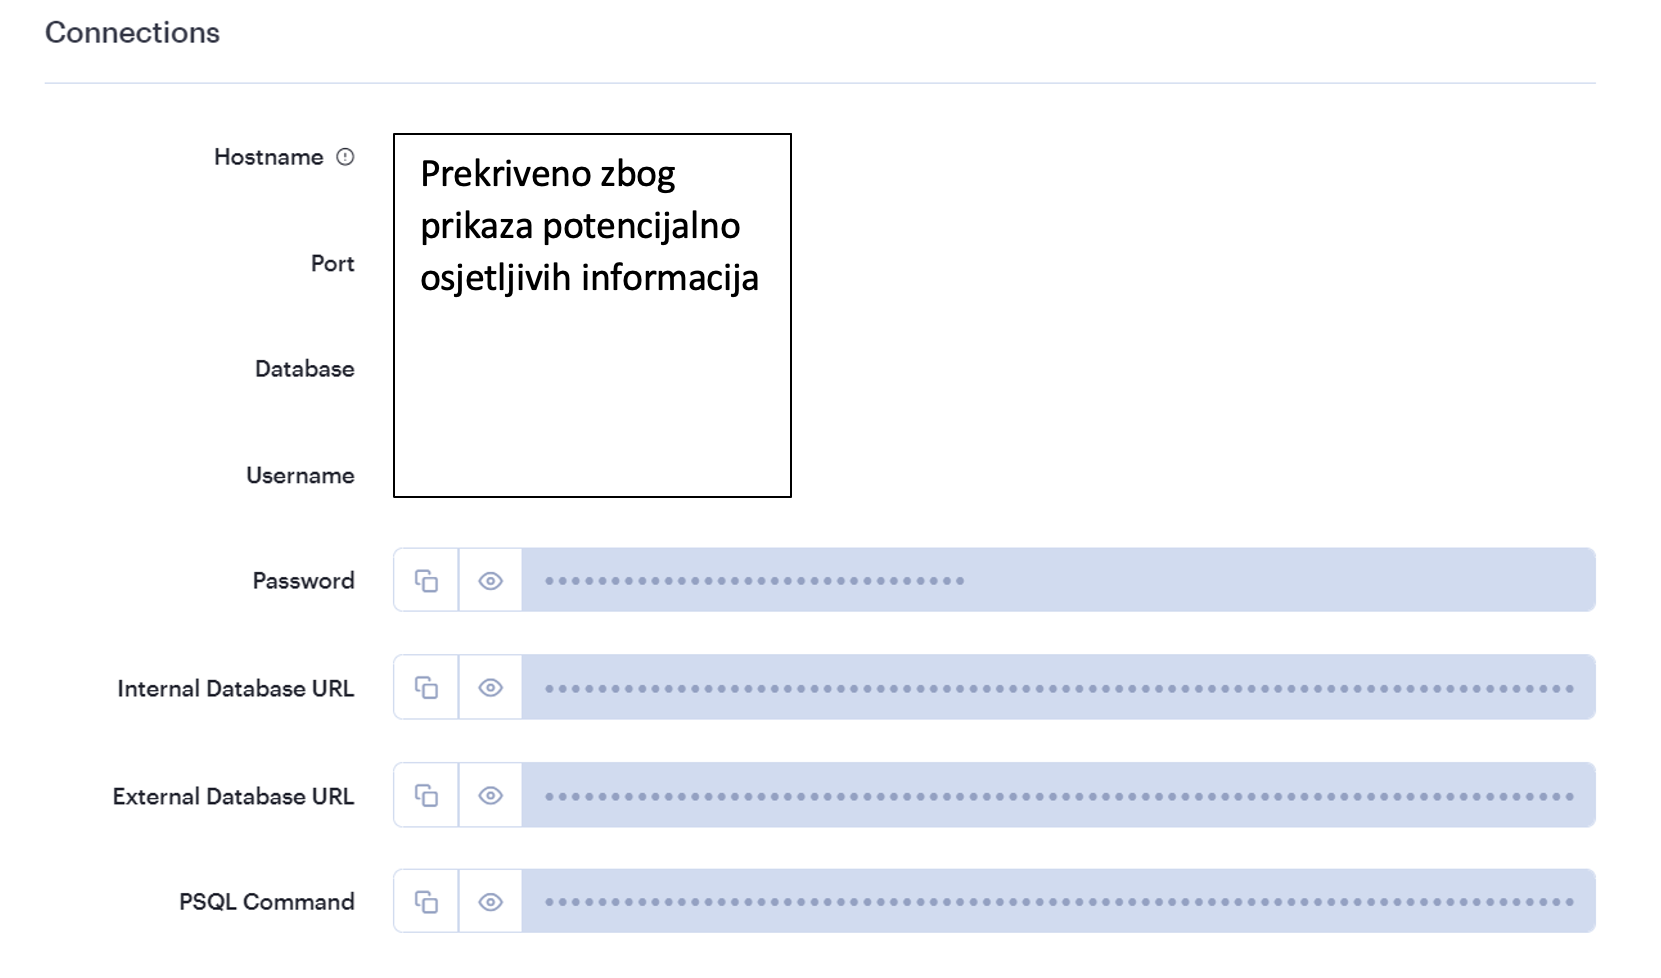
\includegraphics[width=\textwidth]{slike/deployment/slika1.png}
		\caption{Informacije o bazi na Render-u}
		\label{fig:my_label}
    	\end{figure}
    
    \bigskip
    
    	\textbf{\textit{Spajanje pg-Admina s bazom podataka}}\\
		    \textit{Nakon što se instalira pgAdmin potrebno ga je pokrenuti te zatim odabrati opciju „Object“ pa „Register“ pa „Server“ da bi se pojavila forma za spajanje na novu bazu podataka. Prvo,  u polje „Name“ staviti proizvoljno ime baze podataka koje će se prikazati u pgAdmin-u (ne mora biti jednako pravom imenu baze podataka). Nakon toga treba odabrati opciju „Connection“ gdje je potrebno upisati „Host name/address“, „Port“, „Maintenance database“, „Username“ i „Password“, a ostala polja su opcionalna. Za „Username“, „Port“ i „Password“ potrebno je upisati istoimene podatke sa Slike 5.2, za „Maintenance database“ treba staviti podatak „Database“ sa Slike 5.2, a za „Host name/address“ je potrebno staviti dio podatka „External Database URL“ koji se nalazi iza znaka „@“(na kraju se nalazi putanja do baze i iz nje je potrebno izbaciti „/ImeBaze“). Kada su podaci uneseni stisne se gumb „Save“ za spajanje na bazu podataka. Nakon spajanja baza će se vidjeti lijevo na odjelu browser.}
		    
		    \newpage
		 \textbf{\textit{Priprema backend aplikacije za puštanje u pogon}}\\
		 	\textit{U datoteci „application.properties“ potrebno je linije 16-18 zamijeniti linijama 5-9(Slika 5.3). To se radi zato što se baza podataka nalazi u cloud-u što znači da je način spajanja na bazu drugačiji nego kad je ona smještena lokalno. Kod će se nalaziti na javno dostupnom mjestu pa se sigurnost baze podataka poboljšava korištenjem environment varijabli(varijabla tipa \$\{IME\_VARIJABLE\}). Environment varijabla se definira kod stvaranja backend aplikacije i njezinu vrijednost može vidjeti samo vlasnik aplikacije. Osim toga u „application.properties“ treba postaviti „server.servlet.context-path“ na „/spring“ kako bi prefiks zahtjeva na backend aplikaciju bio ispravan te je potrebno dodati datoteku „Dockerfile“ s kodom prikazanim na Slici 5.4 na putanju „./docker/maven/Dockerfile“.}
		   \bigskip
		   \bigskip
         
         \begin{figure}[H]
         	\centering
         	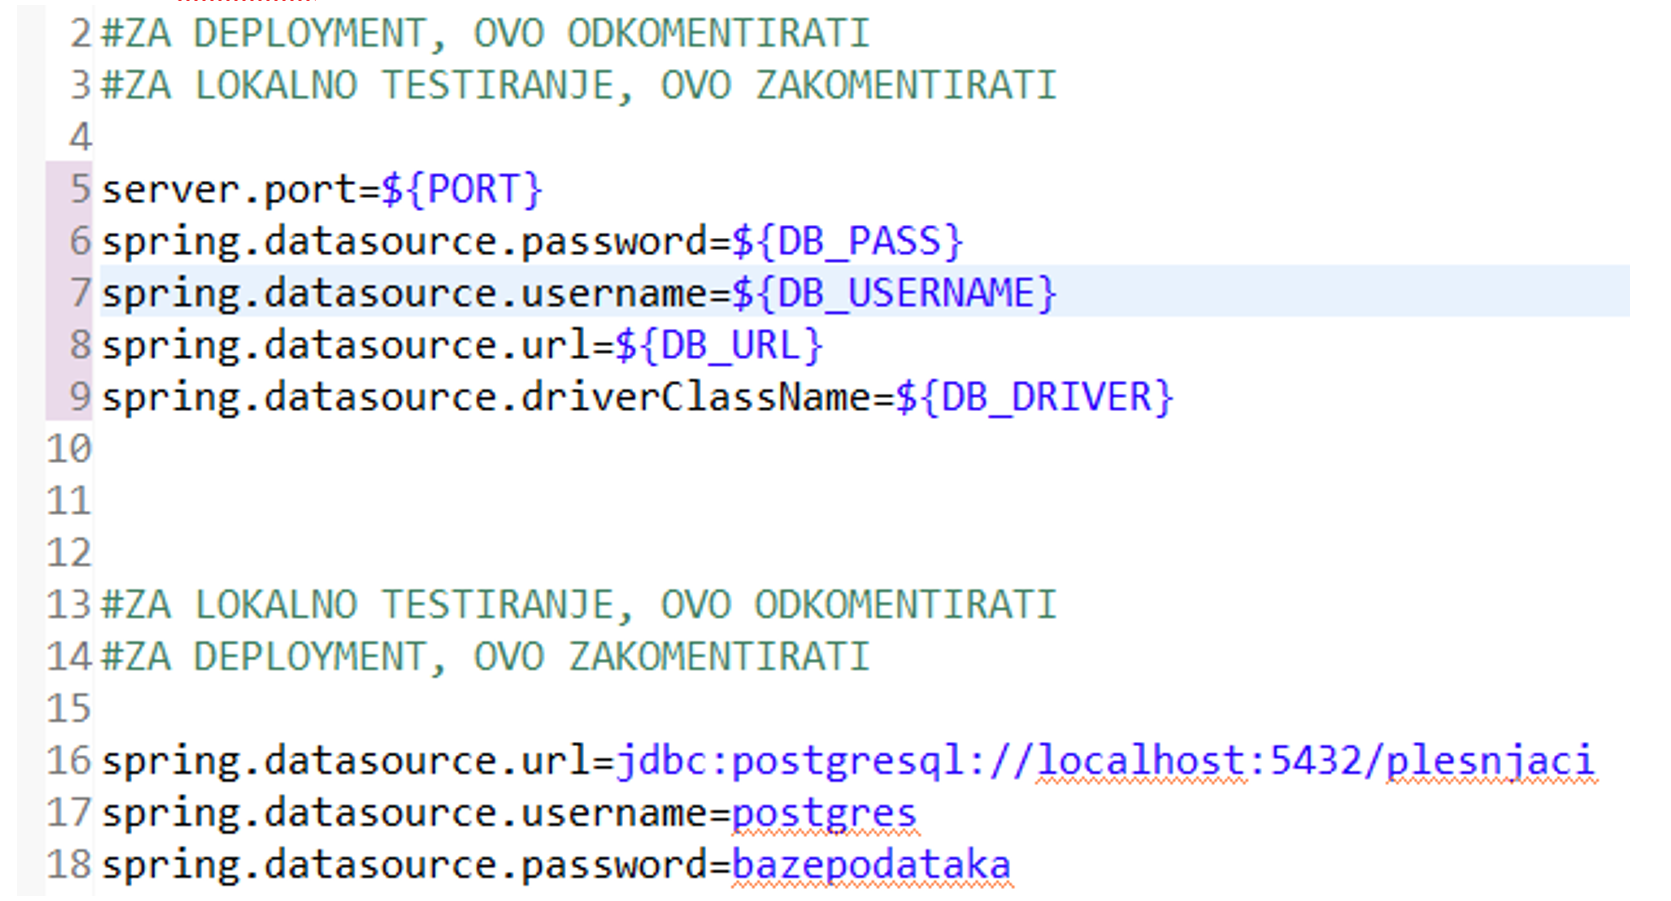
\includegraphics[width=\textwidth]{slike/deployment/slika2.png}
         	\caption{Kod datoteke application.properties}
         	\label{fig:my_label}
         \end{figure}
     
	     \begin{figure}[H]
	     	\centering
	     	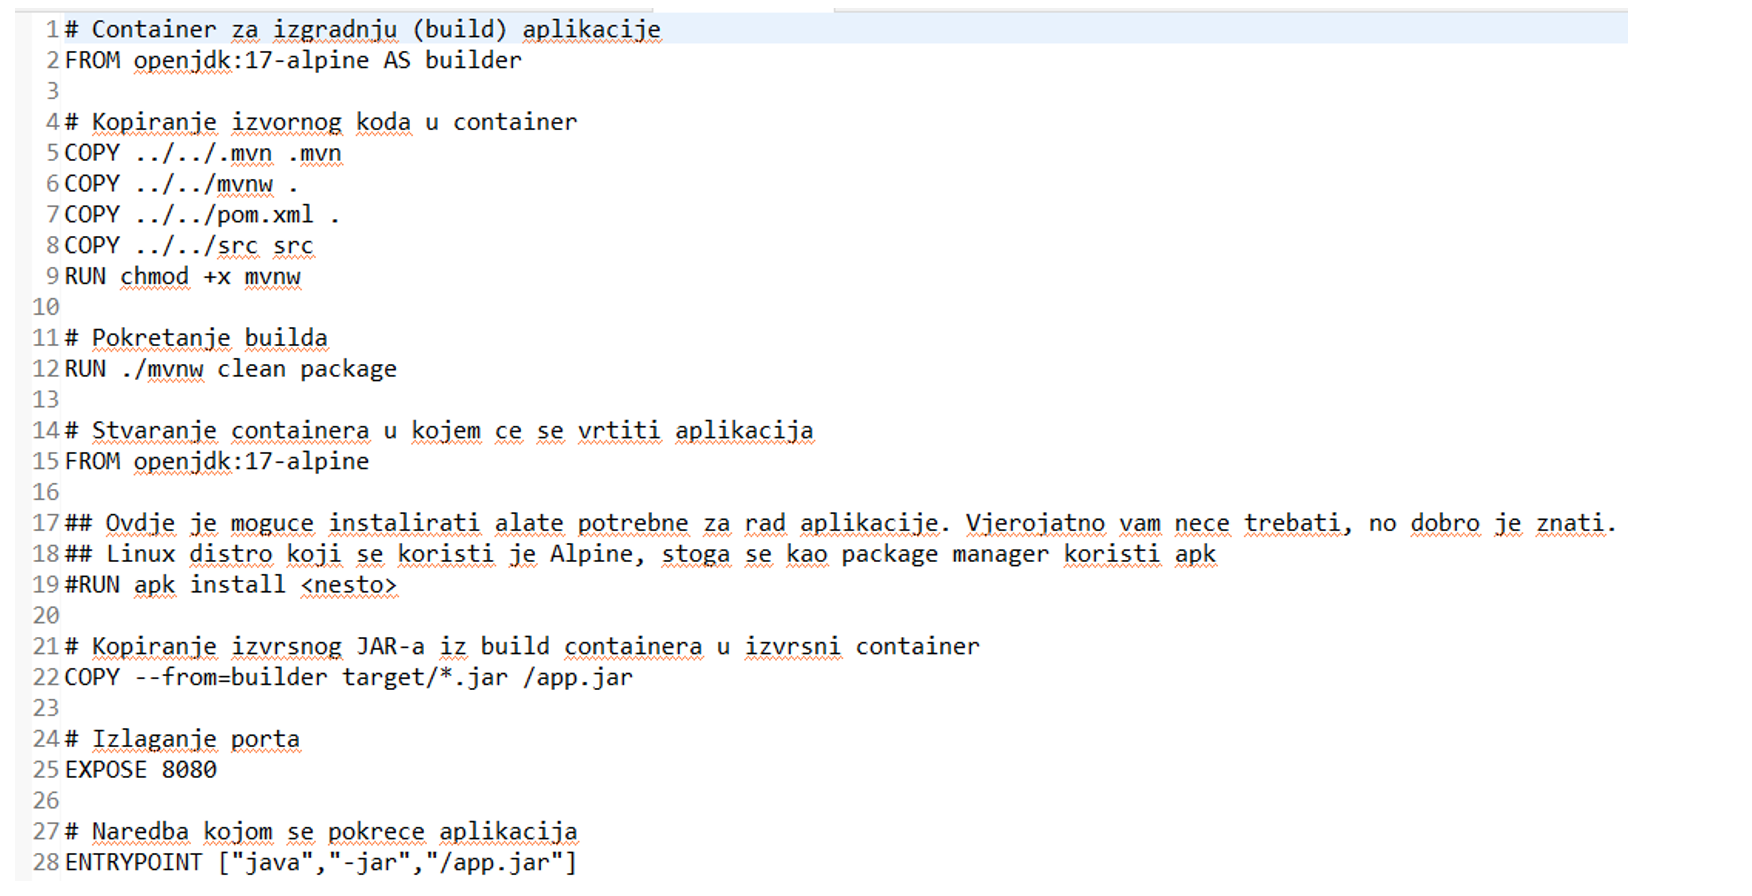
\includegraphics[width=\textwidth]{slike/deployment/slika3.png}
	     	\caption{Kod datoteke Dockerfile}
	     	\label{fig:my_label}
	     \end{figure}
     
        \textbf{\textit{Stvaranje backend aplikacije na Render-u}}\\

       	\textit{Na Render Dashboard-u treba kliknuti na „New“ pa odabrati „Web Service“ da bi se započelo stvaranje web aplikacije. Najprije je potrebno odabrati željeni GitLab repozitorij iz kojeg će se uzimati kod aplikacije klikom na tipku „Connect“ pored imena repozitorija. Na sljedećoj formi potrebno je u polje „Name“ upisati željeno ime aplikacije(ime će postati dio web adrese aplikacije), polje „Region“ treba postaviti na „Frankfurt“, polje „Branch“ postaviti na ime grane GitLab repozitorija s koje se uzima kod aplikacije, u polje „Root Directory“ treba upisati put do koda aplikacije u GitLab repozitoriju(npr. IzvorniKod/SpringBackend/Plesnjaci), postaviti polje „Environment“ na „Docker“ i konačno staviti „Instance Type“ na „Free“. Zatim treba stisnuti na gumb „Advanced“ da bi se otvorila dodatna forma. Na toj formi potrebno je dodati 5 envirnonment varijabli pomoću gumba „Add Environment Variable“ i nazvati ih identično onima na Slici 5.3. Vrijednost varijable „PORT“ su vrata na kojima radi baza podataka, „DB\_URL“ je URL baze podataka u formatu „jdbc:postgresql://hostname:port/database“, „DB\_USERNAME“ je ime vlasnika baze podataka, „DB\_PASS“ je lozinka vlasnika baze podataka, a „DB\_DRIVER“ treba postaviti na „org.postgresql.Driver“. Ukoliko je popunjeno polje „Root Directory“, polja „Docker Build Context Directory“ i „Dockerfile Path“ će imati „Root Directory“ kao prefiks(ako nije popunjeno prefiks se mora ručno dodati), a onda je u ta dva polja potrebno staviti „.“(za prvo) te „./docker/maven/Dockerfile“(za drugo). Ostala polja nije potrebno mijenjati ili popunjavati, a pritiskom na gumb „Create Web Service“ stvara se aplikacija. Novo stvorena aplikacija može se vidjeti na Render Dashboard-u gdje je dostupan i njezin URL.}
       	
       	\bigskip
       	\bigskip
       	
    \textbf{\textit{Priprema frontend aplikacije za puštanje u pogon}}\\
 
    \textit{U datoteci „package.json“ potrebno je u "dependencies" dodati dependancy za http-proxy-middleware, dotenv i express, u "scripts" treba dodati liniju "start-prod": "node app.js" te liniju "build": "react-scripts build" treba zamijeniti s "build": "yarn install \textnormal{\&\&} react-scripts build". Zatim treba dodati datoteku „setupProxy.js“ s kodom prikazanim na Slici 5.5 na putanju „./src/setupProxy.js“ te dodati datoteku „app.js“ s kodom prikazanim na Slici 5.6 na putanju „./app.js“.}
    \bigskip
		    \begin{figure}[H]
		    	\centering
		    	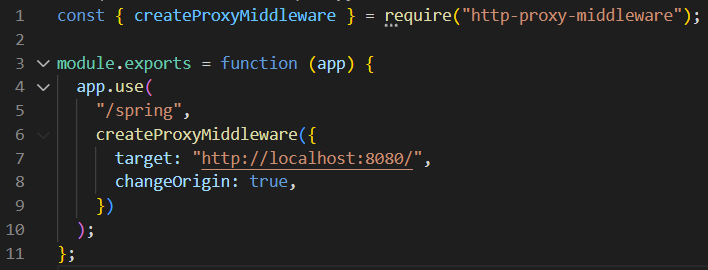
\includegraphics[width=\textwidth]{slike/deployment/slika4.png}
		    	\caption{Kod datoteke setupProxy.js}
		    	\label{fig:my_label}
		    \end{figure}
		
		 \begin{figure}[H]
			\centering
			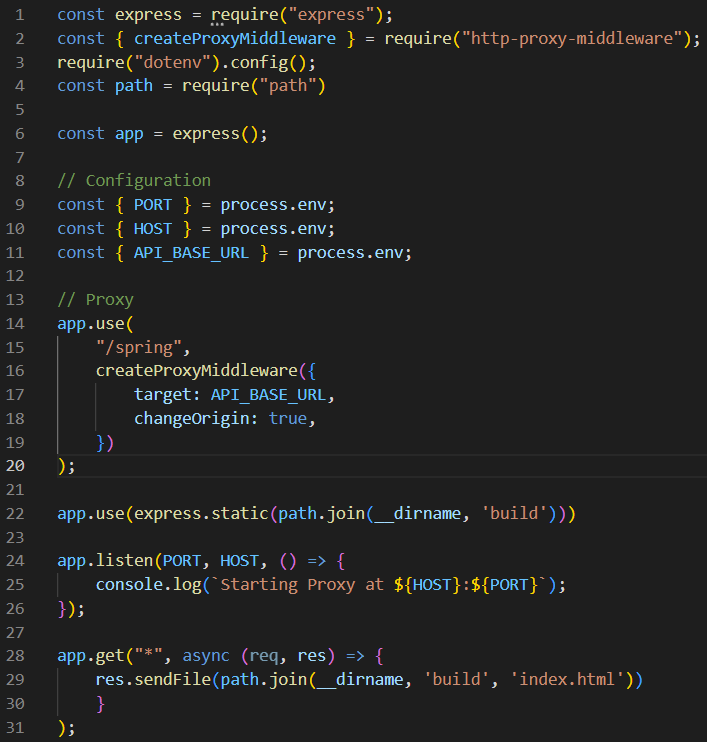
\includegraphics[width=\textwidth]{slike/deployment/slika5.png}
			\caption{Kod datoteke app.js}
			\label{fig:my_label}
		\end{figure}
	
	\newpage
	 \textbf{\textit{Stvaranje frontend aplikacije na Render-u}}\\
	\textit{Na Render Dashboard-u treba kliknuti na „New“ pa odabrati „Web Service“ da bi započelo stvaranje web aplikacije. Najprije je potrebno odabrati željeni GitLab repozitorij iz kojeg će se uzimati kod aplikacije klikom na tipku „Connect“ pored imena repozitorija. Na sljedećoj formi potrebno u polje „Name“ upisati željeno ime aplikacije(ime će postati dio web adrese aplikacije), polje „Region“ treba postaviti na „Frankfurt“, polje „Branch“ postaviti na ime grane GitLab repozitorija s koje se uzima kod aplikacije, u polje „Root Directory“ treba upisati put do koda aplikacije u GitLab repozitoriju(npr. IzvorniKod/ReactFrontend/plesnjaci) i postaviti polje „Envirotnment“ na „Node“. Zatim je potrebno polje „Build Command“ postaviti na „yarn build“ te polje „Start Command“ na „yarn start-prod“. Nakon toga treba stisnuti na gump „Advanced“ da bi se otvorila dodatna forma. Na toj formi potrebno je dodati jednu envirnonment varijablu pomoću gumba „Add Environment Variable“, nazvati ju „API\_BASE\_URL“ i postaviti njezinu vrijednost na URL backend aplikacije na Renderu koji je dostupan na Render Dashboard-u. Ostala polja nije potrebno mijenjati ili popunjavati, a pritiskom na gumb „Create Web Service“ stvara se aplikacija. Novo stvorena aplikacija može se vidjeti na Render Dashboard-u gdje je dostupan i njezin URL.}
	\bigskip
	
	 \textbf{\textit{Pokretanje aplikacije}}\\
	
	\textit{Aplikacija se pokreće upisivanjem linka https://plesnjaci-frontend.onrender.com u browser. Nakon dužeg perioda neaktivnosti aplikacija na Render-u će se automatski ugasiti te će se ponovno podignuti kada primi novi HTTP zahtjev bilo kakve vrste. U takvom slučaju je potrebno pričekati neko vrijeme(najviše nekoliko minuta) dok se aplikacija u potpunosti ne pokrene.}



    

 
	
		
		